% LTeX: language=it

\chapter{Flusso di compilazione}
\label{chap:flusso-di-compilazione}

Nel seguente capitolo si affronteranno, separatamente, le fasi di compilazione di un programma scritto in BugginOut. \`E bene notare che ciascuna di queste fasi prende in ingresso il risultato della fase precedente.

\section{Analisi lessicale}
\label{sec:analisi-lessicale}

Da \cite{alfred2007compilers}:
\begin{parcolumns}[colwidths={1=0.44\textwidth,2=0.44\textwidth},rulebetween=true,nofirstindent=true,sloppy=true]{2}
	% LTeX: language=en_us
	\colchunk{
		\leftskip=1em
		``The main task of the lexical analyzer is to read the input characters of the \emph{source} program, group them into \emph{lexemes}, and produce as output a sequence of \emph{tokens} for each lexeme in the source program.

		[\ldots]

		When discussing lexical analysis, we use three related but distinct terms:
		\begin{itemize}
			\item A \emph{token} is a pair consisting of a token \emph{name} and an optional attribute \emph{value}. The token name is an abstract symbol representing a kind of lexical unit, e.g., a particular keyword, or a sequence of input characters denoting an identifier. [\ldots]
			\item A \emph{pattern} is a description of the form that the lexemes of a token may take. In the case of a kewyord as a token, the pattern is just the sequence of characters that form the keyword. For identifiers and some other tokens, the pattern is a more complex structure that is matched by many strings.
			\item A \emph{lexeme} is a sequence of characters in the source program that matches the pattern for a token and is identified by the lexical analyzer as an instance of that token.
		\end{itemize}
	}
	% LTeX: language=it
	\colchunk{
		\leftskip=1em
		``Il compito principale di un analizzatore lessicale \`e la lettura dei caratteri di input del programma \emph{sorgente}, raggrupparli in \emph{lessemi} e produrre, come risultato, una sequenza di \emph{token} per ogni lessema del programma sorgente.

		[\ldots]

		Durante la discussione dell'analisi lessicale, si usano tre legati ma distinti termini:
		\begin{itemize}
			\item Un \emph{token} \`e una coppia costituita di un \emph{nome} e un \emph{valore} opzionale. Il nome \`e un simbolo astratto che rappresenta il tipo di unit\`a lessicale, ad esempio, una particolare parola chiave oppure una sequenza di caratteri che denota un identificatore. [\dots]
			\item Un \emph{pattern} \`e una descrizione della forma che i lessemi di un token possono avere. Nel caso di una parola chiave come token, il pattern \`e semplicemente la sequenza di caratteri che formano la parola chiave. Per gli identificatori e qualche altro token, il pattern \`e una struttura pi\`u complessa che riconosce pi\`u stringhe.
			\item Un \emph{lessema} \`e una sequenza di caratteri del programma sorgente.''
		\end{itemize}
	}
	\colplacechunks
\end{parcolumns}

\begin{table}[H]
	\begin{tabularx}{\textwidth}{X|X|X}
		\hline
		\hline
		\multicolumn{1}{c|}{\textsc{Token}} & \multicolumn{1}{c|}{\textsc{Pattern} (informale)} & \multicolumn{1}{c}{\textsc{Lessemi}} \\
		\hline
		\texttt{kw\_for} & i seguenti caratteri: \texttt{for} & \texttt{for} \\
		\hline
		\texttt{kw\_if} & i seguenti caratteri: \texttt{if} & \texttt{if} \\
		\hline
		\texttt{Identifier} & una lettera oppure \mbox{\texttt{\_} o \texttt{\$}} seguita da una serie di lettere, cifre numeriche oppure \mbox{\texttt{\_} o \texttt{\$}} & \texttt{a}, \texttt{b}, \texttt{token\_name}, \texttt{num1}, \ldots \\
		\hline
		\texttt{IntegerLiteral} & uno o pi\`u cifre decimali\footnotemark & \texttt{1}, \texttt{123}, \ldots \\
		\hline
		\hline
	\end{tabularx}
	\caption{Alcuni token di BugginOut}
	\label{fig:bugginout-example-tokens}
\end{table}

\footnotetext{In BugginOut \`e possibile utilizzare i numeri in notazione binari, ottale ed esadecimale. Per esempio \texttt{0b101} \`e un numero binario, \texttt{0o127} \`e un numero ottale e \texttt{0x1A} \`e un numero esadecimale. Inoltre possono essere seguiti da un suffisso per indicarne il tipo. Il pattern per entrambi \`e stato omesso in quanto non rilevante per l'esempio.}

Nella fase di analisi lessicale si alternano due operazioni:
\begin{itemize}
	\item definita da \cite{alfred2007compilers} come \emph{scanning}, si ignorano i caratteri che non sono significativi per il linguaggio (spazi bianchi e \emph{commenti});
	\item definita da \cite{alfred2007compilers} come \emph{lexical analysis}, \`e la parte pi\`u complessa in cui si producono i token.
\end{itemize}

Quando pi\`u di un lessema pu\`o essere riconosciuto da un pattern, l'analizzatore lessicale inserisce nel valore delle informazioni aggiuntive utili alle fasi successive di compilazione. Ad esempio, nel caso di un numero, il valore \`e il numero stesso. Ad esempio, facendo riferimento all'esempio \ref{fig:bugginout-example-tokens}, il token \texttt{IntegerLiteral} conterrebbe come valore \texttt{123}.

\`E importante osservare che ci\`o che influenzer\`a le decisioni di analisi grammaticale del compilatore \`e il nome del token e non il suo valore che, invece, viene usato per la traduzione dei token.

Per completezza, di seguito verranno riportati tutti i token definiti in BugginOut.
\begin{xltabular}{\textwidth}{l|X}
	\caption{Token di BugginOut}
	\label{fig:bugginout-complete-tokens} \\

	\hline
	\hline
	\multicolumn{1}{c|}{\textsc{Token}} & \multicolumn{1}{c|}{\textsc{Pattern} (in POSIX ERE \cite{iso-9945-2009})} \\
	\hline
	\endfirsthead

	\hline
	\multicolumn{1}{c|}{\textsc{Token}} & \multicolumn{1}{c|}{\textsc{Pattern}} \\
	\hline
	\endhead

	\endfoot

	\hline
	\hline
	\endlastfoot

	\texttt{kw\_anon} & \texttt{anon} \\ \hline
	\texttt{kw\_as} & \texttt{as} \\ \hline
	\texttt{kw\_bool} & \texttt{bool} \\ \hline
	\texttt{kw\_break} & \texttt{break} \\ \hline
	\texttt{kw\_char} & \texttt{char} \\ \hline
	\texttt{kw\_continue} & \texttt{continue} \\ \hline
	\texttt{kw\_else} & \texttt{else} \\ \hline
	\texttt{kw\_f32} & \texttt{f32} \\ \hline
	\texttt{kw\_f64} & \texttt{f64} \\ \hline
	\texttt{kw\_false} & \texttt{false} \\ \hline
	\texttt{kw\_fn} & \texttt{fn} \\ \hline
	\texttt{kw\_for} & \texttt{for} \\ \hline
	\texttt{kw\_i16} & \texttt{i16} \\ \hline
	\texttt{kw\_i32} & \texttt{i32} \\ \hline
	\texttt{kw\_i64} & \texttt{i64} \\ \hline
	\texttt{kw\_i8} & \texttt{i8} \\ \hline
	\texttt{kw\_if} & \texttt{if} \\ \hline
	\texttt{kw\_in} & \texttt{in} \\ \hline
	\texttt{kw\_isize} & \texttt{isize} \\ \hline
	\texttt{kw\_mut} & \texttt{mut} \\ \hline
	\texttt{kw\_null} & \texttt{null} \\ \hline
	\texttt{kw\_return} & \texttt{return} \\ \hline
	\texttt{kw\_true} & \texttt{true} \\ \hline
	\texttt{kw\_u16} & \texttt{u16} \\ \hline
	\texttt{kw\_u32} & \texttt{u32} \\ \hline
	\texttt{kw\_u64} & \texttt{u64} \\ \hline
	\texttt{kw\_u8} & \texttt{u8} \\ \hline
	\texttt{kw\_usize} & \texttt{usize} \\ \hline
	\texttt{kw\_var} & \texttt{var} \\ \hline
	\texttt{kw\_void} & \texttt{void} \\ \hline
	\texttt{Ampersand} & \texttt{\&} \\ \hline
	\texttt{AmpersandEquals} & \texttt{\&=} \\ \hline
	\texttt{Asterisk} & \texttt{*} \\ \hline
	\texttt{AsteriskEquals} & \texttt{*=} \\ \hline
	\texttt{At} & \texttt{@} \\ \hline
	\texttt{BinaryLiteral} & \texttt{0b[01]+(\_[a-zA-Z\_\$][a-zA-Z\_\$0-9]*)?}  \\ \hline
	\texttt{CharLiteral} & \texttt{\textquotesingle([\textasciicircum \textquotesingle \textbackslash \textbackslash]|\textbackslash \textbackslash \textquotesingle |\textbackslash \textbackslash n|\textbackslash \textbackslash r|\textbackslash \textbackslash t|\textbackslash\textbackslash\textbackslash\textbackslash|\textbackslash \textbackslash 0|\textbackslash \textbackslash x[0-7][0-9a-fA-F])\textquotesingle} \\ \hline
	\texttt{Circumflex} & \texttt{\textbackslash\textasciicircum} \\ \hline
	\texttt{CircumflexEquals} & \texttt{\textbackslash\textasciicircum=} \\ \hline
	\texttt{Colon} & \texttt{:} \\ \hline
	\texttt{Comma} & \texttt{,} \\ \hline
	\texttt{DecimalLiteral} & \texttt{[0-9]+(\_[a-zA-Z\_\$][a-zA-Z\_\$0-9]*)?} \\ \hline
	\texttt{Dot} & \texttt{\textbackslash .} \\ \hline
	\texttt{DotDotEquals} & \texttt{\textbackslash .\textbackslash .=} \\ \hline
	\texttt{DotDotLessThan} & \texttt{\textbackslash .\textbackslash .<} \\ \hline
	\texttt{DoubleAmpersand} & \texttt{\&\&} \\ \hline
	\texttt{DoubleAmpersandEquals} & \texttt{\&\&=} \\ \hline
	\texttt{DoubleEquals} & \texttt{==} \\ \hline
	\texttt{DoublePipe} & \texttt{\textbackslash |\textbackslash |} \\ \hline
	\texttt{DoublePipeEquals} & \texttt{\textbackslash |\textbackslash |=} \\ \hline
	\texttt{EndOfFile} & Non ha un pattern associato in quanto viene generato quando l'analizzatore lessicale ha terminato di analizzare il programma sorgente. \\ \hline
	\texttt{Equals} & \texttt{=} \\ \hline
	\texttt{ExclamationMark} & \texttt{!} \\ \hline
	\texttt{ExclamationMarkEquals} & \texttt{!=} \\ \hline
	\texttt{FloatLiteral} & \texttt{[0-9]+\textbackslash.[0-9]+(\_[a-zA-Z\_\$][a-zA-Z\_\$0-9]*)?} \\ \hline
	\texttt{GreaterThan} & \texttt{>} \\ \hline
	\texttt{GreaterThanEquals} & \texttt{>=} \\ \hline
	\texttt{HexadecimalLiteral} & \texttt{0x[0-9a-fA-F]+(\_[a-zA-Z\_\$][a-zA-Z\_\$0-9]*)?} \\ \hline
	\texttt{Identifier} & \texttt{[a-zA-Z\_\$][a-zA-Z\_\$0-9]*} \\ \hline
	\texttt{LeftCurlyBracket} & \texttt{\{} \\ \hline
	\texttt{LeftParenthesis} & \texttt{\textbackslash (} \\ \hline
	\texttt{LeftShift} & \texttt{<<} \\ \hline
	\texttt{LeftShiftEquals} & \texttt{<<=} \\ \hline
	\texttt{LeftSquareBracket} & \texttt{\textbackslash \char"5B} \\ \hline
	\texttt{LessThan} & \texttt{<} \\ \hline
	\texttt{LessThanEquals} & \texttt{<=} \\ \hline
	\texttt{Minus} & \texttt{-} \\ \hline
	\texttt{MinusEquals} & \texttt{-=} \\ \hline
	\texttt{MinusMinus} & \texttt{--} \\ \hline
	\texttt{OctalLiteral} & \texttt{0o[0-7]+(\_[a-zA-Z\_\$][a-zA-Z\_\$0-9]*)?} \\ \hline
	\texttt{Percent} & \texttt{\%} \\ \hline
	\texttt{PercentEquals} & \texttt{\%=} \\ \hline
	\texttt{Pipe} & \texttt{\textbackslash |} \\ \hline
	\texttt{PipeEquals} & \texttt{\textbackslash |=} \\ \hline
	\texttt{Plus} & \texttt{+} \\ \hline
	\texttt{PlusEquals} & \texttt{+=} \\ \hline
	\texttt{PlusPlus} & \texttt{++} \\ \hline
	\texttt{RightCurlyBracket} & \texttt{\}} \\ \hline
	\texttt{RightParenthesis} & \texttt{\textbackslash )} \\ \hline
	\texttt{RightShift} & \texttt{>>} \\ \hline
	\texttt{RightShiftEquals} & \texttt{>>=} \\ \hline
	\texttt{RightSquareBracket} & \texttt{\textbackslash ]} \\ \hline
	\texttt{Semicolon} & \texttt{;} \\ \hline
	\texttt{Solidus} & \texttt{/} \\ \hline
	\texttt{SolidusEquals} & \texttt{/=} \\ \hline
	\texttt{StringLiteral} & \texttt{\textquotedbl ([\textasciicircum \textquotedbl \textbackslash \textbackslash]|\textbackslash \textbackslash \textquotedbl|\textbackslash \textbackslash n|\textbackslash \textbackslash r|\textbackslash \textbackslash t|\textbackslash \textbackslash \textbackslash \textbackslash|\textbackslash \textbackslash 0|\textbackslash \textbackslash x[0-7][0-9a-fA-F])*\textquotedbl} \\ \hline
	\texttt{Tilde} & \texttt{\textasciitilde}
\end{xltabular}
Per riconoscere i token, si passa dai pattern ad una rappresentazione intermedia: i \textit{transition diagram}. Questi vengono definiti da \cite{alfred2007compilers} e non sono altro che degli automi a stati finiti.
\begin{figure}[H]
	\centering
	\begin{tikzpicture}[node distance=3.5cm, on grid, auto]
		\node[state, initial] (0) {$q_0$};
		\node[state, accepting] (1) [right=of 0] {$q_1$};

		\path[->]
		(0) edge node {\texttt{[a-zA-Z\_\$]}} (1)
		(1) edge [loop above] node {\texttt{[a-zA-Z\_\$0-9]}} ();
	\end{tikzpicture}
	\caption{Diagramma di transizione per il token \texttt{Identifier}}
	\label{fig:bugginout-identifier-transition-diagram}
\end{figure}
Questo diagramma di transizione \`e composto da due stati: lo stato iniziale $q_0$ e lo stato finale $q_1$. Quando il diagramma \`e in uno stato finale, significa che il token \`e stato riconosciuto.

In questo caso, il diagramma inizia dallo stato $q_0$ e si sposta nello stato finale $q_1$ quando incontra un carattere che corrisponde al pattern. Da questo punto in poi, il diagramma rimane nello stato finale fino a quando non incontra un carattere che non corrisponde al pattern.

Un esempio pi\`u complesso \`e quello del riconoscimento dei numeri (i token \texttt{BinaryLiteral}, \texttt{OctalLiteral}, \texttt{HexadecimalLiteral}, \texttt{DecimalLiteral} e \texttt{FloatLiteral}):
\begin{figure}[H]
	\centering
	\scalebox{0.6}{\begin{tikzpicture}[node distance=3.5cm, on grid, auto]
		\node[state, initial] (0) {$q_0$};
		\node[state] (1) [right=of 0] {$q_1$};
		\node[state] (2) [right=of 1] {$q_2$};
		\node[state] (3) [below=of 2] {$q_3$};
		\node[state] (4) [below=of 3] {$q_4$};
		\node[state, accepting] (5) [right=of 2] {$q_5$};
		\node[state] (6) [right=of 5] {$q_6$};
		\node[state, accepting] (7) [right=of 6] {$q_7$};
		\node[state, accepting] (8) [right=of 3] {$q_8$};
		\node[state] (9) [right=of 8] {$q_9$};
		\node[state, accepting] (10) [right=of 9] {$q_{10}$};
		\node[state, accepting] (11) [right=of 4] {$q_{11}$};
		\node[state] (12) [right=of 11] {$q_{12}$};
		\node[state, accepting] (13) [right=of 12] {$q_{13}$};
		\node[state, accepting] (14) [below=10.5cm of 1] {$q_{14}$};
		\node[state] (15) [right=of 14] {$q_{15}$};
		\node[state, accepting] (16) [right=of 15] {$q_{16}$};
		\node[state] (17) [right=of 16] {$q_{17}$};
		\node[state, accepting] (18) [right=of 17] {$q_{18}$};
		\node[state] (19) [below=of 15] {$q_{19}$};
		\node[state, accepting] (20) [right=of 19] {$q_{20}$};

		\path[->]
		(0) edge node {\texttt{0}} (1)
		(1) edge node {\texttt{b}} (2)
		(1) edge node {\texttt{o}} (3)
		(1) edge node {\texttt{x}} (4)
		(1) edge node {\texttt{[0-9]}} (14)
		(2) edge node {\texttt{[01]}} (5)
		(5) edge [loop above] node {\texttt{[01]}} ()
		(5) edge node {\texttt{\_}} (6)
		(6) edge node {\texttt{[a-zA-Z\_\$]}} (7)
		(7) edge [loop above] node {\texttt{[a-zA-Z\_\$0-9]}} ()
		(3) edge node {\texttt{[0-7]}} (8)
		(8) edge [loop above] node {\texttt{[0-7]}} ()
		(8) edge node {\texttt{\_}} (9)
		(9) edge node {\texttt{[a-zA-Z\_\$]}} (10)
		(10) edge [loop above] node {\texttt{[a-zA-Z\_\$0-9]}} ()
		(4) edge node {\texttt{[0-9a-fA-F]}} (11)
		(11) edge [loop above] node {\texttt{[0-9a-fA-F]}} ()
		(11) edge node {\texttt{\_}} (12)
		(12) edge node {\texttt{[a-zA-Z\_\$]}} (13)
		(13) edge [loop above] node {\texttt{[a-zA-Z\_\$0-9]}} ()
		(0) edge node {\texttt{[1-9]}} (14)
		(14) edge [loop left] node {\texttt{[0-9]}} ()
		(14) edge node {\texttt{.}} (15)
		(15) edge node {\texttt{[0-9]}} (16)
		(16) edge [loop above] node {\texttt{[0-9]}} ()
		(16) edge node {\texttt{\_}} (17)
		(17) edge node {\texttt{[a-zA-Z\_\$]}} (18)
		(18) edge [loop above] node {\texttt{[a-zA-Z\_\$0-9]}} ()
		(14) edge node {\texttt{\_}} (19)
		(19) edge node {\texttt{[a-zA-Z\_\$]}} (20)
		(20) edge [loop above] node {\texttt{[a-zA-Z\_\$0-9]}} ();
	\end{tikzpicture}}
	\caption{Diagramma di transizione per i token numerici}
	\label{fig:bugginout-number-transition-diagram}
\end{figure}

In questo caso:
\begin{itemize}
	\item $q_5$ e $q_7$ sono gli stati finali per \texttt{BinaryLiteral};
	\item $q_8$ e $q_{10}$ sono gli stati finali per \texttt{OctalLiteral};
	\item $q_{11}$ e $q_{13}$ sono gli stati finali per \texttt{HexadecimalLiteral};
	\item $q_{14}$ e $q_{20}$ sono gli stati finali per \texttt{DecimalLiteral};
	\item $q_{16}$ e $q_{18}$ sono gli stati finali per \texttt{FloatLiteral}.
\end{itemize}

Si possono costruire diagrammi di transizione per ogni token e, inoltre, \`e possibile unirli per averne uno solo che rappresenter\`a l'intero funzionamento dell'analizzatore lessicale.

\section{Analisi grammaticale}
\label{sec:analisi-grammaticale}

L'analisi grammaticale costituisce la fase in cui la sequenza di token prodotta dall'analisi lessicale viene organizzata secondo le regole sintattiche del linguaggio, definite da una \emph{grammatica} formale. Lo scopo di questa fase \`e costruire una struttura ad albero, l'\emph{AST} (\textit{Abstract Syntax Tree}), che rappresenta gerarchicamente la struttura del programma. Ogni nodo di questo albero rappresenta un costrutto sintattico del linguaggio, come espressioni, dichiarazioni o blocchi di codice. Compito di questa fase \`e anche individuare gli \emph{errori sintattici} come, ad esempio, parentesi non bilanciate o costrutti mal formati.

Per definire il comportamento dell'analizzatore grammaticale \`e necessario definire la grammatica del linguaggio definita da \cite{alfred2007compilers}:
\begin{parcolumns}[colwidths={1=0.44\textwidth,2=0.44\textwidth},rulebetween=true,nofirstindent=true,sloppy=true]{2}
	% LTeX: language=en_us
	\colchunk{
		\leftskip=1em
		``A context-free grammar (grammar for short) consists of \emph{terminals}, \emph{nonterminals}, a \emph{start symbol} and \emph{productions}.

		\begin{itemize}
			\item \emph{Terminals} are the basic symbols from which strings are formed. The term "token name" is a synonim for "terminal" [\ldots].
			\item \emph{Nonterminals} are syntactic variables that denote sets of strings. [\dots]. Nonterminals impose a hierarchical structure on the language that is key to syntax analysis and translation.
			\item In a grammar, one nonterminal is distinguished as the \emph{start symbol}, and the set of strings it denotes is the language generated by the grammar. [\ldots]
			\item The productions of a grammar specify the manner in which the terminals and nonterminals can be combined to form strings. Each \emph{production} consists of:
			\begin{itemize}
				\item A nonterminal called the \emph{head} or \emph{left side} of the production; this production defines some of the strings denoted by the head.
				\item{} [\ldots]
				\item A \emph{body} or \emph{right side} consisting of zero or more terminals and nonterminals. The components of the body describe one way in which strings of the nonterminal at the head can be constructed.''
			\end{itemize}
		\end{itemize}
	}
	% LTeX: language=it
	\colchunk{
		\leftskip=1em
		``Una grammatica context-free (grammatica in breve) \`e costituita da \emph{terminali}, \emph{non terminali}, un \emph{simbolo di partenza} e da \emph{produzioni}.

		\begin{itemize}
			\item I \emph{terminali} sono i simboli di base da cui sono formate le stringhe. Il termine "nome del token" \`e sinonimo di "terminale" [\ldots].
			\item I \emph{non terminali} sono variabili sintattiche che denotano insiemi di stringhe. [\ldots]. I non terminali impongono una struttura gerarchica al linguaggio che \`e fondamentale per l'analisi sintattica e la traduzione.
			\item In una grammatica, un non terminale \`e distinto come il \emph{simbolo di partenza} e l'insieme di stringhe che denota \`e il linguaggio generato dalla grammatica. [\ldots]
			\item Le produzioni di una grammatica specificano il modo in cui i terminali e i non terminali possono essere combinati per formare stringhe. Ogni \emph{produzione} \`e costituita da:
			\begin{itemize}
				\item Un non terminale chiamato \emph{testa} o \emph{lato sinistro} della produzione; questa produzione definisce alcune delle stringhe denotate dalla testa.
				\item{} [\ldots]
				\item Un \emph{corpo} o \emph{lato destro} costituito da zero o pi\`u terminali e non terminali. I componenti del corpo descrivono un modo in cui le stringhe del non terminale nella testa possono essere costruite.''
			\end{itemize}
		\end{itemize}
	}
	\colplacechunks
\end{parcolumns}

\`E bene notare che questo tipo di grammatica non \`e capace di descrivere l'intera sintassi del linguaggio. Ad esempio, il requisito che una variabile sia dichiarata prima del suo utilizzo o che il valore assegnatogli sia del tipo corretto non pu\`o essere descritto in questo modo. Questo tipo di controlli \`e compito della fase di analisi semantica (vedi la sezione \ref{sec:analisi-semantica}).

Vediamo alcuni costrutti sintattici di BugginOut scritti in BNF (\textit{Backus-Naur Form}).

\begin{figure}[H]
	\centering
	\begin{minted}[breaklines,frame=lines,fontsize=\footnotesize]{text}
<function_parameter> ::= "anon"? "mut"? <Identifier> ":" <Type>
<function_parameters> ::= <function_parameter> ("," <function_parameter>)*

<FunctionDeclarationStatement> ::=
  "fn" <Identifier> "(" <function_parameters>? ")" ":" <Type>
  <BlockExpression>
  \end{minted}
	\label{fig:bugginout-function-declaration}
	\caption{Grammatica per la dichiarazione di una funzione}
\end{figure}

In questo esempio possiamo notare che una dichiarazione di funzione \`e definita, in ordine, da:
\begin{itemize}
	\item la parola chiave \texttt{fn};
	\item un'identificatore (il token \texttt{Identifier});
	\item una parentesi tonda aperta (il token \texttt{LeftParenthesis});
	\item una lista opzionale di parametri definiti dalla regola \raggedright\texttt{<function\_parameters>};
	\item una parentesi tonda chiusa (il token \texttt{RightParenthesis});
	\item due punti (il token \texttt{Colon});
	\item un tipo, definito dalla regola \texttt{<Type>};
	\item un blocco, definito dalla regola \texttt{<BlockExpression>}.
\end{itemize}

A loro volta, i parametri della funzione sono definiti da un parametro di funzione, definito dalla regola \texttt{<function\_parameter>}, seguito da una virgola e da un altro parametro di funzione ripetuti zero o pi\`u volte. \`E importante osservare che la ricorsione \`e destra e non sinistra; il motivo verr\`a approfondito quando si discuter\`a del tipo di approccio utilizzato per l'analisi grammaticale.

Avendone discusso la grammatica vediamo, ad esempio, la dichiarazione una semplice funzione per sommare due numeri interi.
\begin{figure}[H]
	\centering
	\begin{minted}[breaklines,linenos,frame=lines,fontsize=\footnotesize]{text}
fn add(a: i32, b: i32): i32 {
  a + b
}
	\end{minted}
	\label{fig:bugginout-example-function-declaration}
	\caption{Semplice dichiarazione di funzione in BugginOut}
\end{figure}

L'analizzatore grammaticale, per la funzione dichiarata nell'esempio precedente, generer\`a il seguente AST:\footnote{Nell'AST riportato \`e stato omesso, per ogni nodo, il figlio \texttt{span} che non \`e rilevante per la sua analisi (si veda il capitolo \ref{chap:architettura-del-compilatore}).}
\begin{figure}[H]
	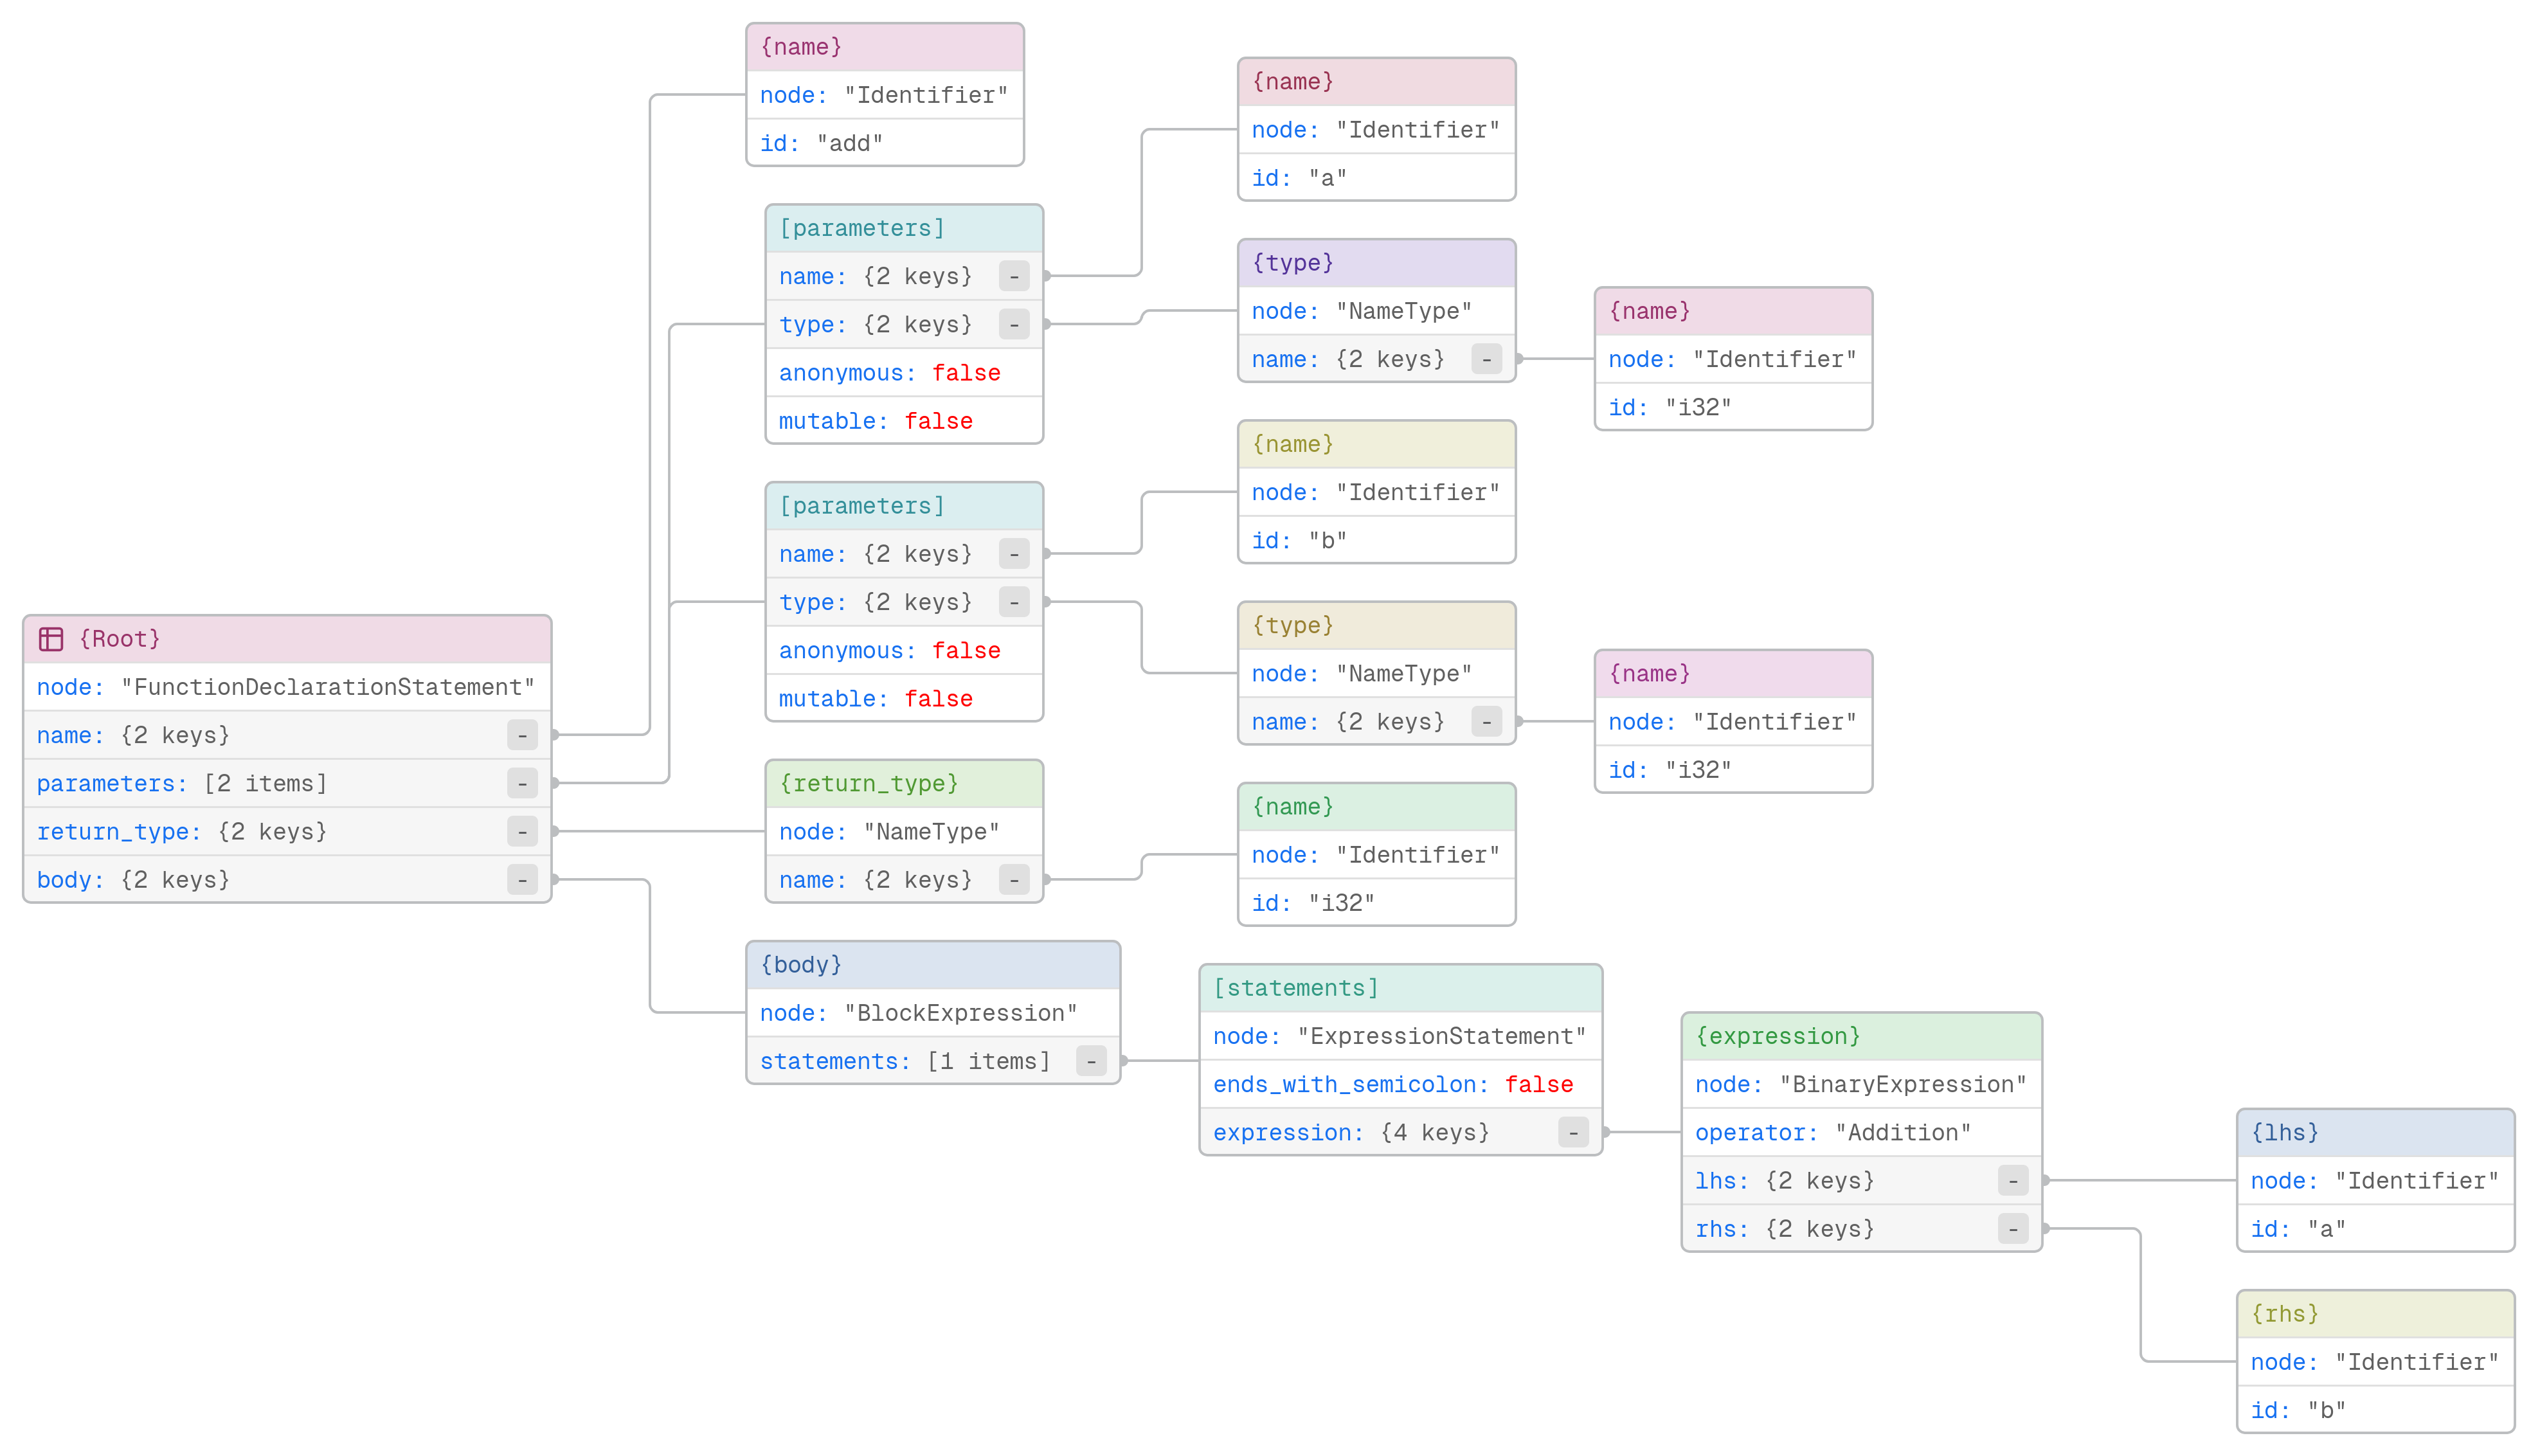
\includegraphics[width=\textwidth]{figures/function_declaration_ast.png}
	\label{fig:bugginout-example-function-declaration-ast}
	\caption{AST generato per la funzione nell'esempio precedente}
\end{figure}
Come possiamo vedere, la radice \`e il nodo \texttt{FunctionDeclarationStatement} che ha come figli:
\begin{itemize}
	\item \texttt{name} (un \texttt{Identifier}): nome della funzione;
	\item \texttt{function\_parameters}: i parametri della funzione, i cui figli sono due nodi, uno per ogni parametro, con a loro volta come figli:
	\begin{itemize}
		\item \texttt{name} (un \texttt{Identifier}): nome del parametro;
		\item \texttt{type} (un \texttt{Type}): tipo del parametro;
		\item \texttt{mutable}: se il parametro \`e mutabile o meno;
		\item \texttt{anonymous}: se il parametro \`e anonimo o meno.
	\end{itemize}
	\item \texttt{return\_type} (un \texttt{Type}): il tipo di ritorno della funzione;
	\item \texttt{body} (una \texttt{BlockExpression}): il corpo della funzione che ha come foglia il nodo \texttt{BinaryExpression} che rappresenta l'espressione \texttt{a + b} e ha come figli:
	\begin{itemize}
		\item \texttt{operator}: che rappresenta l'operatore dell'espressione (in questo caso una somma);
		\item \texttt{lhs} (una \texttt{Expression}, in questo caso specifico un \texttt{Identifier}): la parte sinistra dell'operazione;
		\item \texttt{rhs} (una \texttt{Expression}, in questo caso specifico un \texttt{Identifier}): la parte destra dell'operazione.
	\end{itemize}
\end{itemize}

Un altro esempio interessante \`e la definizione delle espressioni binarie:
\begin{figure}[H]
	\centering
	\begin{minted}[breaklines,frame=lines,fontsize=\footnotesize]{text}
<BinaryExpression> ::=
  <Expression>
  ("+" | "-" | "*" | "/" | "%" | "<<" | ">>" | "<" | ">" | "<=" | ">=" | "==" | "!=" | "&" | "^" | "|" | "&&" | "||")
  <Expression>
	\end{minted}
	\label{fig:bugginout-binary-expression}
	\caption{Grammatica per le espressioni binarie}
\end{figure}

Il motivo per cui ci interessa analizzare questa regola \`e la sua \emph{ambiguit\`a}, ci\`o significa che esistono pi\`u modi d'interpretare la stessa espressione. Ad esempio, l'espressione \texttt{a + b * c} pu\`o essere interpretata in due modi diversi:
\begin{itemize}
	\item \texttt{(a + b) * c}, in cui l'operazione di somma viene eseguita prima della moltiplicazione;
	\item \texttt{a + (b * c)}, in cui l'operazione di moltiplicazione viene eseguita prima della somma.
\end{itemize}
Citando \cite{alfred2007compilers}:
\begin{parcolumns}[colwidths={1=0.44\textwidth,2=0.44\textwidth},rulebetween=true,nofirstindent=true,sloppy=true]{2}
	% LTeX: language=en_us
	\colchunk{
		\leftskip=1em
		``There are two reasons why we might prefer to use the ambiguous grammar. [\ldots] We can easily change the \emph{associativity} and \emph{precedence} of the operators without disturbing the productions or the number of states in the resulting parser.~[\ldots]''
	}
	% LTeX: language=it
	\colchunk{
		\leftskip=1em
		``Ci sono due ragioni per le quali potremmo preferire utilizzare la grammatica ambigua. [\ldots] Possiamo facilmente cambiare l'\emph{associatività} e \emph{precedenza} degli operatori senza disturbare le produzioni o il numero di stati dell'analizzatore grammaticale.~[\ldots]''
	}
	\colplacechunks
\end{parcolumns}

Chiarito il concetto di grammatica e avendone visto alcuni esempi, \`e possibile passare alla discussione dell'analizzatore grammaticale.

In generale un analizzatore grammaticale pu\`o seguire due principali strategie:
\begin{itemize}
	\item \emph{top-down}, in cui l'analizzatore grammaticale inizia dalla radice dell'albero e scende verso le foglie;
	\item \emph{bottom-up}, in cui l'analizzatore grammaticale inizia dalle foglie dell'albero e risale verso la radice.
\end{itemize}
La strategia scelta per BugginOut \`e quella \emph{top-down} per la sua semplicit\`a e facilit\`a d'uso. Pi\`u specificamente, l'analizzatore lessicale \`e un \textit{predictive parser} senza \textit{backtracking} costruito su una grammatica LL(1) \cite{alfred2007compilers}.

Questo significa che, a ogni passo, si sceglie la produzione grammaticale corretta utilizzando solo il prossimo token restituito dall'analizzatore lessicale. \`E importante notare che, per costruire un analizzatore grammaticale di questo tipo, \`e necessario che la grammatica sia priva di \emph{ambiguit\`a} e \emph{ricorsioni sinistre}. La prima condizione \`e stata soddisfatta definendo l'associativit\`a e la precedenza degli operatori\footnote{Lo si vede nel dettaglio nel capitolo \ref{chap:architettura-del-compilatore}.} e la seconda scrivendo meticolosamente la grammatica per evitarle.

Durante l'analisi grammaticale, si potrebbe incorrere in un errore sintattico se un token incontrato durante l'analisi lessicale del programma sorgente non corrisponde a quello che ci si aspetta nella produzione.
\begin{figure}[H]
	\centering
	\begin{minted}[breaklines,linenos,frame=lines,fontsize=\footnotesize]{text}
fn add(a: i32, b: i32): i32 {
  (a + b
}
	\end{minted}
	\begin{minted}[breaklines,frame=lines,fontsize=\footnotesize]{text}
error.bo: Expected "RightParenthesis", got "RightCurlyBracket"!
   3 | }
       ^
	\end{minted}
	\label{fig:bugginout-syntax-error}
	\caption{Errore sintattico generato nel caso di parentesi non bilanciate}
\end{figure}
In questo caso l'analizzatore grammaticale genera un errore e termina l'esecuzione. Questo approccio di gestione degli errori \`e il pi\`u semplice e non \`e in grado di recuperare gli errori\footnote{Su questo tema si spenderanno alcune parole nella sezione \ref{sec:limiti}.}.

\section{Analisi semantica}
\label{sec:analisi-semantica}

L'analisi semantica \`e la fase di compilazione in cui viene verificata la correttezza semantica del programma. In questa fase, l'analizzatore semantico controlla che le operazioni siano valide in base al tipo di dati e alle regole del linguaggio.

I controlli semantici includono:
\begin{itemize}
	\item ordine delle dichiarazioni: verifica che le variabili siano dichiarate prima di essere utilizzate;
	\item ambito (\emph{scope}): verifica che le variabili siano utilizzate all'interno del loro ambito di visibilit\`a;
	\item assegnabilit\`a: verifica se un'espressione \`e assegnabile ad un'altra;
	\item firma delle funzioni: verifica che le funzioni siano chiamate con il numero e il tipo corretto di argomenti;
	\item ...
\end{itemize}
Di tutti i controlli quello che merita una particolare attenzione \`e il \emph{type checking} (controllo dei tipi). Questo controllo verifica che i valori siano usati in maniera coerenti con i loro tipi, ad esempio che non si tenti di assegnare un numero a una stringa o che si assegni un valore booleano a una variabile intera.

Citando \cite{alfred2007compilers}:
\begin{parcolumns}[colwidths={1=0.44\textwidth,2=0.44\textwidth},rulebetween=true,nofirstindent=true,sloppy=true]{2}
	% LTeX: language=en_us
	\colchunk{
		\leftskip=1em
		``To do \emph{type checking} a compiler needs to assign a type expression to each component of the source program. The compiler must then determine that these type expressions conform to a collection of logical rules that is called the \emph{type system} for the source language.

		[\ldots]

		Type checking can take on two forms: synthesis and inference. \emph{Type synthesis} builds up the type of an expression from the types of its sub expressions.~[\dots] \emph{Type inference} determines the type of a language construct from the way it is used.''
	}
	% LTeX: language=it
	\colchunk{
		\leftskip=1em
		``Per fare il \emph{type checking} un compilatore deve assegnare un'espressione di tipo a ciascun componente del programma sorgente. Il compilatore deve quindi determinare che queste espressioni di tipo siano conformi a una collezione di regole logiche che viene chiamata \emph{type sistem} per il linguaggio sorgente.

		[\ldots]

		Il type checking pu\`o assumere due forme: sintesi e inferenza. La \emph{sintesi} costruisce il tipo di un'espressione dai tipi delle sue sottoespressioni.~[\dots] L'\emph{inferenza} determina il tipo di un costrutto del linguaggio dal modo in cui viene utilizzato.''
	}
	\colplacechunks
\end{parcolumns}

Analizziamo ora alcuni esempi di \emph{type checking}.

Di seguito le operazioni per l'analisi semantica di una dichiarazione di variabile:
\begin{enumerate}
	\item si verifica se la dichiarazione specifica un tipo per la variabile in maniera esplicita:
	\begin{itemize}
		\item in tal caso, si passa ad analizzare semanticamente l'espressione che inizializza la variabile e a verificare che abbia lo stesso tipo della variabile (esempio di sintesi del tipo della variabile);
		\item altrimenti, la variabile assume il valore del tipo dell'espressione che la inizializza (esempio d'inferenza del tipo della variabile).
	\end{itemize}
	\item si verifica se la variabile \`e gi\`a stata dichiarata in precedenza usando la \emph{tabella dei simboli}\footnote{Si veda il capitolo \ref{chap:architettura-del-compilatore} per un approfondimento su questo argomento.}.
\end{enumerate}

Di seguito le operazioni per l'analisi semantica di un'espressione \texttt{if}:
\begin{enumerate}
	\item si esegue l'analisi semantica della condizione e si verifica che il tipo dell'espressione sia booleana;
	\item si esegue l'analisi semantica del blocco \texttt{then};
	\item se esiste, si esegue l'analisi semantica del blocco \texttt{else} e si controlla che abbia lo stesso tipo del blocco \texttt{then}.
\end{enumerate}

Di seguito le operazioni per l'analisi semantica di un'espression \texttt{return}:
\begin{enumerate}
	\item si verifica se si restituisce un'espressione:
	\begin{itemize}
		\item in tal caso, si esegue l'analisi semantica dell'espressione e si verifica che il suo tipo sia compatibile con il tipo di ritorno della funzione che si sta analizzando;
		\item altrimenti, si verifica che la funzione abbia tipo di ritorno \texttt{void}.
	\end{itemize}
\end{enumerate}

Durante le operazioni descritte si possono generare errori semantici. Ad esempio, se si tenta di dichiarare una variabile con lo stesso nome di una gi\`a esistente, si genera un errore semantico.

Osserviamone ora qualche esempio:
\begin{figure}[H]
	\centering
	\begin{minted}[breaklines,linenos,frame=lines,fontsize=\footnotesize]{text}
fn add(a: i32): i32 {
  var c = a + b;
  return c;
}
	\end{minted}
	\begin{minted}[breaklines,frame=lines,fontsize=\footnotesize]{text}
not_declared.bo: Unknown identifier
   2 |   var c = a + b;
                     ^
	\end{minted}
	\label{fig:unknown-identifier-error}
	\caption{Errore semantico generato per una variabile non dichiarata}
\end{figure}

\begin{figure}[H]
	\centering
	\begin{minted}[breaklines,linenos,frame=lines,fontsize=\footnotesize]{text}
fn foo(): i32 {
	return 1 + "2";
}
	\end{minted}
	\begin{minted}[breaklines,frame=lines,fontsize=\footnotesize]{text}
invalid_operation.bo: Incompatible types for binary operation
   2 |   return 1 + "2";
                ^^^^^^^
	\end{minted}
	\label{fig:invalid-binary-operation-error}
	\caption{Errore semantico generato per un'operazione non valida}
\end{figure}

\begin{figure}[H]
	\centering
	\begin{minted}[breaklines,linenos,frame=lines,fontsize=\footnotesize]{text}
fn foo(): i32 {
	return "10";
}
	\end{minted}
	\begin{minted}[breaklines,frame=lines,fontsize=\footnotesize]{text}
invalid_return.bo: Incompatible return types
   2 |     return "10";
           ^^^^^^^^^^^^
	\end{minted}
	\label{fig:invalid-return-type-error}
	\caption{Errore semantico generato per un tipo di ritorno non valido}
\end{figure}

\`E importante notare che gli errori semantici sono corretti dal punto di vista della grammatica del linguaggio, ma violano la logica del linguaggio. Trovare questi errori in fase di compilazione, prima dell'esecuzione di un programma, rende il codice pi\`u robusto e riduce il rischio di comportamenti imprevisti.

\section{Generazione del codice}
\label{sec:generazione-del-codice}

La generazione del codice \`e la fase finale della compilazione in cui si traduce il \texttt{CheckedAST} (output dell'analisi semantica) in codice C++ pronto per essere compilato. Il codice generato in C++ ha l'obiettivo di essere leggibile e quanto pi\`u vicino possibile a quello originale, in modo da facilitarne il debug.

Il codice C++ generato \`e composto da:
\begin{itemize}
	\item \emph{prelude}: una serie di dichiarazioni e inclusioni necessarie per il corretto funzionamento del codice generato\footnote{Lo si approfondir\`a nel capitolo \ref{chap:architettura-del-compilatore}.};
	\item prototipi delle funzioni: per ogni funzione dichiarata nel programma BugginOut originale, ne si inserisce il prototipo;
	\item dichiarazioni di funzioni: dopo averne dichiarato i prototipi, si passa a inserirne le implementazioni;
	\item \emph{main}: la funzione principale del programma, costituita da una sola chiamata alla funzione \emph{bo\_main}\footnote{La funzione \texttt{main} deve essere presente in ogni programma BugginOut e in fase di generazione del codice viene rinominata in \texttt{bo\_main} per evitare conflitti con la funzione \texttt{main} prevista dal compilatore C++}.
\end{itemize}

Sebbene una quantit\`a elevata dei nodi generati trova una corrispondenza diretta con il codice C++ generato, alcuni nodi meritano un particolare approfondimento: i tipi, l'espressioni \texttt{if} e i blocchi.

Per la traduzione dei tipi, si effettuano le seguenti operazioni:
\begin{itemize}
	\item i tipi primitivi vengono tradotti cos\`i come sono grazie a degli alias definiti dal \emph{prelude};
	\item gli \emph{array} vengono tradotti in \texttt{std::array};
	\item gli \emph{slice} vengono tradotti in \texttt{std::span};
	\item i range vengono tradotti nel tipo \texttt{bo\_range} definito nel \emph{prelude}\footnote{Si veda il capitolo \ref{chap:architettura-del-compilatore} per un approfondimento su questo tipo.};
	\item i puntatori vengono tradotti usando la sintassi dei puntatori C++ (ovvero \texttt{type*})\footnote{\`E bene notare che quindi un puntatore, \emph{weak} o \emph{strong} che sia, viene tradotto nello stesso tipo. \`E possibile farlo in quanto la compatibilit\`a dei tipi \`e garantita dalla fase di analisi semantica.};
\end{itemize}

Le espressioni \texttt{if}, invece, meritano un trattamento speciale nel caso in cui queste siano usate come espressione, ad esempio se si deve tradurre:
\begin{figure}[H]
	\centering
	\begin{minted}[breaklines,frame=lines,fontsize=\footnotesize]{text}
var x = if (a > b) { a } else { b };
	\end{minted}
	\label{fig:bugginout-if-expression}
	\caption{Esempio di espressione \texttt{if} in BugginOut usata come espressione}
\end{figure}
Per tradurre questo tipo di espressione, non supportata nativamente dal C++, si fa uso dell'estensione \emph{compound statements} del compilatore GNU\footnote{Di questo si parler\`a meglio nel capitolo \ref{chap:conclusioni}.} per tradurre l'espressione in un blocco di codice che restituisce il valore corretto:
\begin{figure}[H]
	\centering
	\begin{minted}[breaklines,frame=lines,fontsize=\footnotesize]{cpp}
i32 const x = (({
    i32 __block_ret_1 {};
    if (static_cast<bool>((a)>(b)))
    {
        __block_ret_1 = a;
    }
    else
    {
        __block_ret_1 = ({
            b;
        });
    }
    __block_ret_1;
}));
	\end{minted}
	\label{fig:bugginout-if-expression-transpiled}
	\caption{Traduzione dell'esempio precedente in C++}
\end{figure}
In questo modo, l'espressione \texttt{if} viene tradotta in un blocco di codice che memorizza il valore corretto in una variabile restituita alla fine di esso.

Un discorso analogo vale per i blocchi di codice, per fare un esempio, il seguente blocco di codice
\begin{figure}[H]
	\centering
	\begin{minted}[breaklines,frame=lines,fontsize=\footnotesize]{text}
var y = {
    var x = 1;
    x + 2
}
	\end{minted}
	\label{fig:bugginout-block-expression}
	\caption{Esempio di blocco che restituisce un valore in BugginOut}
\end{figure}
viene tradotto in C++ come:
\begin{figure}[H]
	\centering
	\begin{minted}[breaklines,frame=lines,fontsize=\footnotesize]{cpp}
i32 const y = ({
    i32 const x = (static_cast<i32>(1));
    static_cast<i32>((x)+(static_cast<i32>(2)));
});
	\end{minted}
	\label{fig:bugginout-block-expression-transpiled}
	\caption{Traduzione dell'esempio precedente in C++}
\end{figure}

Una volta generato il codice C++, questo viene memorizzato in un file con estensione \texttt{.cpp} e, successivamente, compilato usando il compilatore GNU C++ per produrre un eseguibile\footnote{Si veda il capitolo \ref{chap:architettura-del-compilatore} per un approfondimento su questo argomento.}.
